\section{Scalability}
\label{sec:scalability}

\subsection{Current posture}
\status{INFERRED}

The stateless JWT design allows horizontal scaling of the Spring Boot tier, but the single MySQL instance, file-less local state, and absence of caching, read replicas, or async processing bound vertical growth. No horizontal-scaling configuration (compose file, replica policy, migration runner) exists in the repository.

\begin{figure}[H]
\centering
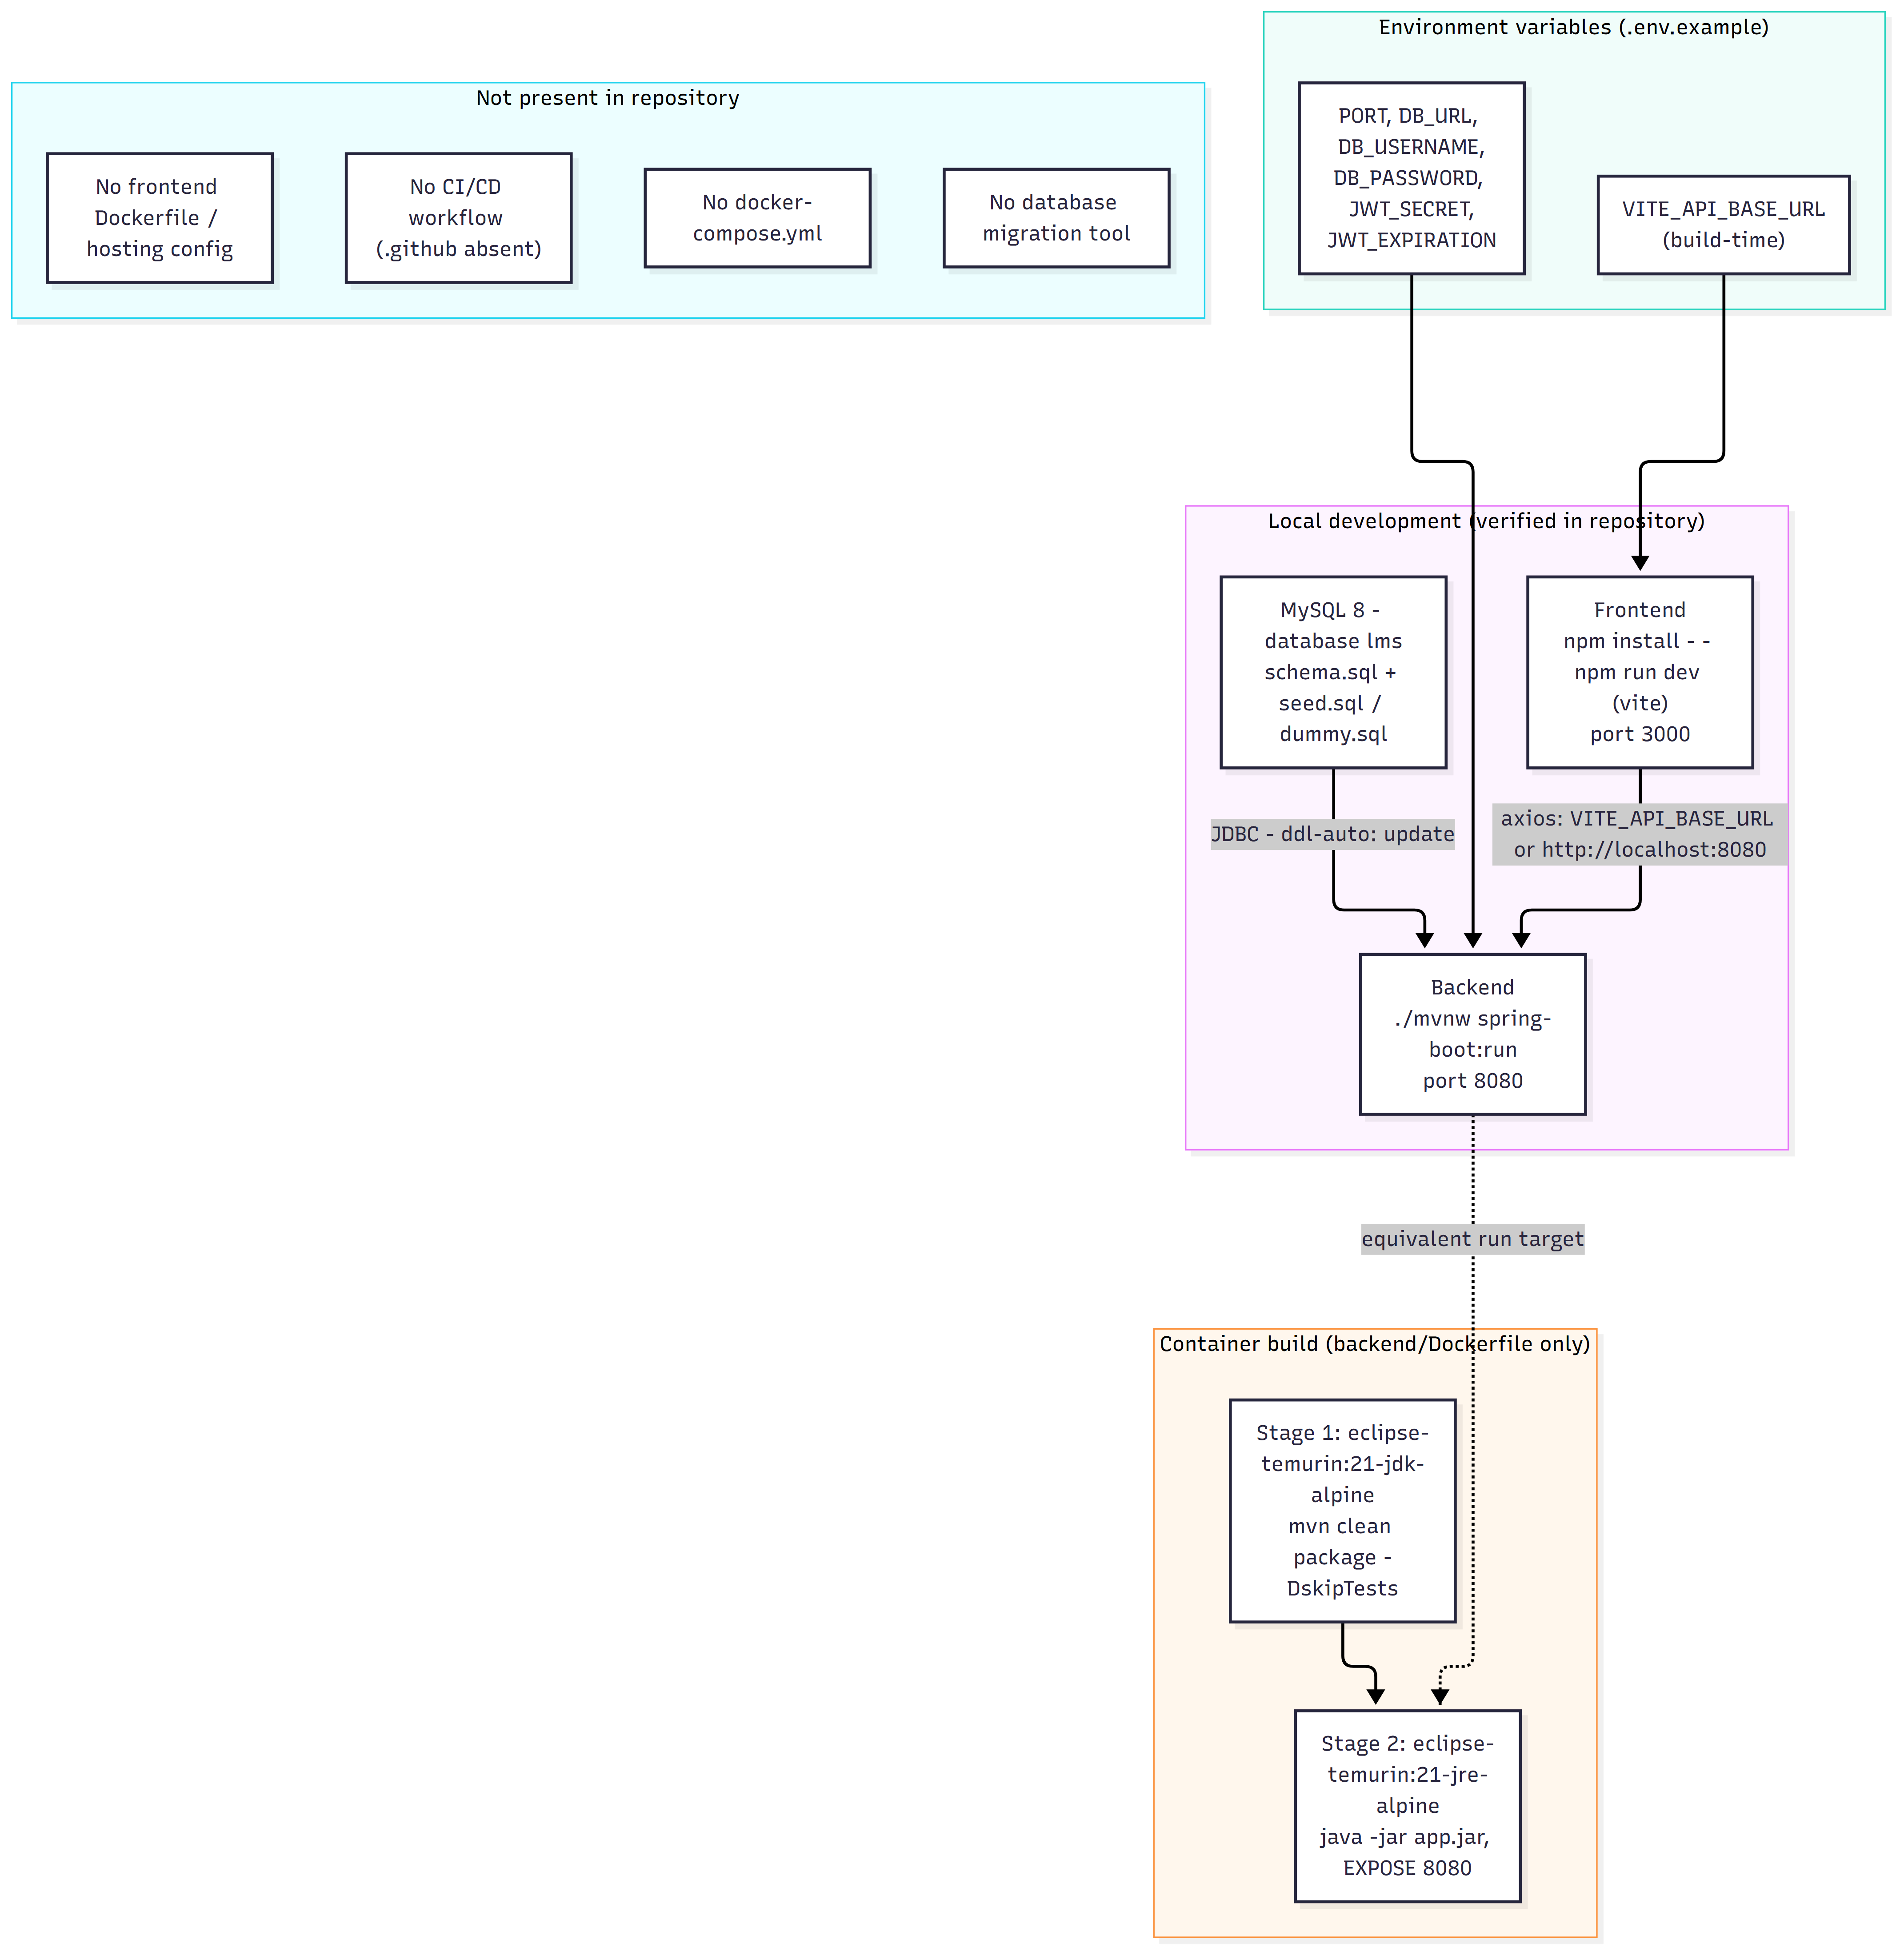
\includegraphics[width=0.9\textwidth]{diagrams/deployment.png}
\caption{Deployment view -- the only containerised component is the backend JAR}
\label{fig:deployment}
\end{figure}

\subsection{Scaling path}
\status{RECOMMENDED}

Containerise the frontend static bundle, add a compose or orchestrator topology, externalise sessions only if introduced, adopt versioned migrations before multi-instance deploys, then consider read replicas, caching, and CDN for static assets. Do not claim elastic scalability until the database and migration story are hardened.
